\documentclass{article}
\usepackage{listings}
\usepackage{graphicx}
\usepackage{color}

\definecolor{mygreen}{rgb}{0,0.6,0}
\definecolor{mygray}{rgb}{0.5,0.5,0.5}
\definecolor{mymauve}{rgb}{0.58,0,0.82}

\lstset{ %
  backgroundcolor=\color{white},   % choose the background color; you must add \usepackage{color} or \usepackage{xcolor}; should come as last argument
  basicstyle=\footnotesize,        % the size of the fonts that are used for the code
  breakatwhitespace=false,         % sets if automatic breaks should only happen at whitespace
  breaklines=true,                 % sets automatic line breaking
  captionpos=b,                    % sets the caption-position to bottom
  commentstyle=\color{mygreen},    % comment style
  deletekeywords={...},            % if you want to delete keywords from the given language
  escapeinside={\%*}{*)},          % if you want to add LaTeX within your code
  extendedchars=true,              % lets you use non-ASCII characters; for 8-bits encodings only, does not work with UTF-8
  frame=single,	                   % adds a frame around the code
  keepspaces=true,                 % keeps spaces in text, useful for keeping indentation of code (possibly needs columns=flexible)
  keywordstyle=\color{blue},       % keyword style
  language=Octave,                 % the language of the code
  morekeywords={*,...},           % if you want to add more keywords to the set
  numbers=left,                    % where to put the line-numbers; possible values are (none, left, right)
  numbersep=5pt,                   % how far the line-numbers are from the code
  numberstyle=\tiny\color{mygray}, % the style that is used for the line-numbers
  rulecolor=\color{black},         % if not set, the frame-color may be changed on line-breaks within not-black text (e.g. comments (green here))
  showspaces=false,                % show spaces everywhere adding particular underscores; it overrides 'showstringspaces'
  showstringspaces=false,          % underline spaces within strings only
  showtabs=false,                  % show tabs within strings adding particular underscores
  stepnumber=2,                    % the step between two line-numbers. If it's 1, each line will be numbered
  stringstyle=\color{mymauve},     % string literal style
  tabsize=2,	                   % sets default tabsize to 2 spaces
  title=\lstname                   % show the filename of files included with \lstinputlisting; also try caption instead of title
}

\author{Jacob Hutter}
\title{ECE 311 Lab 4}

\begin{document}
\maketitle
\color{red}
\underline{\textbf{Report Item 1}}
\color{black}
\lstinputlisting[language=Matlab]{filters.m}
\begin{figure}[H]
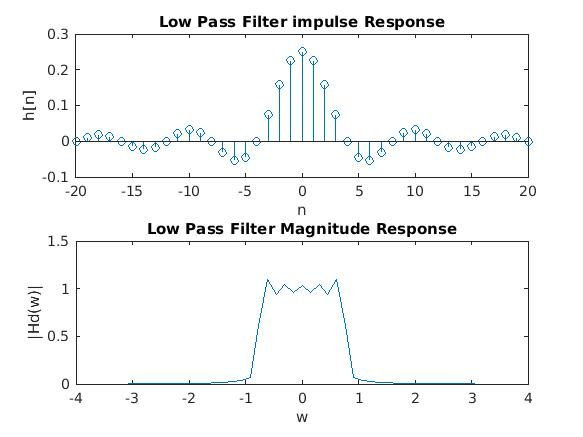
\includegraphics[scale = .5]{1_lpf_20}
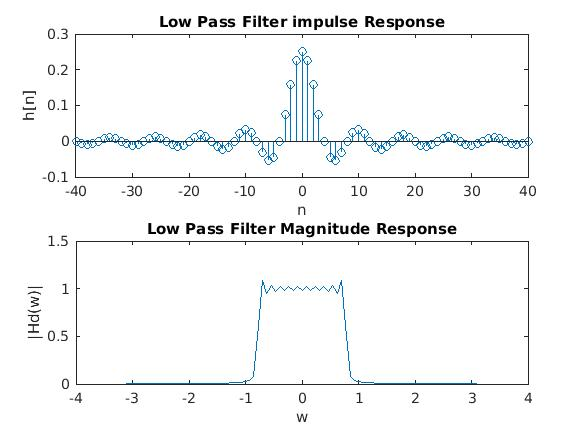
\includegraphics[scale = .5]{1_lpf_40}
\\ Notice that the magnitude response shows some attenuation and non-vertical edges that would not be present in an ideal model of a filter. This is not possible in a setting with a discrete amount of samples because the jump from low to high or vice versa happens instantaneously.
\end{figure}

\begin{figure}[H]
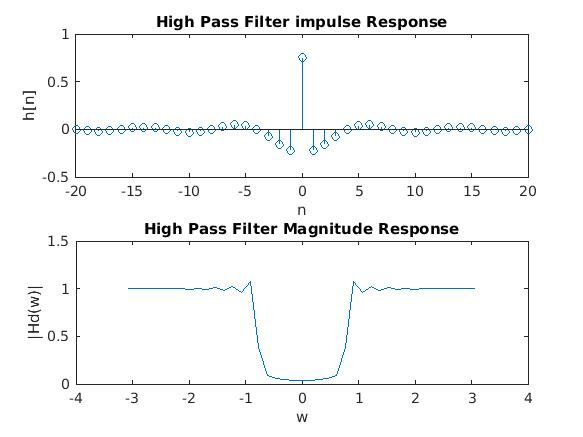
\includegraphics[scale = .5]{1_hpf_20}
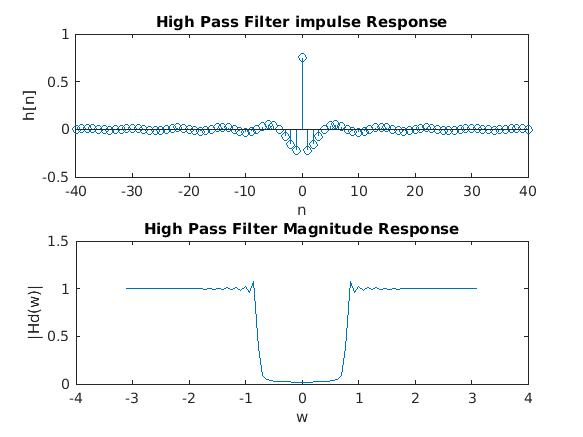
\includegraphics[scale = .5]{1_hpf_40}
\end{figure}
\begin{figure}[H]
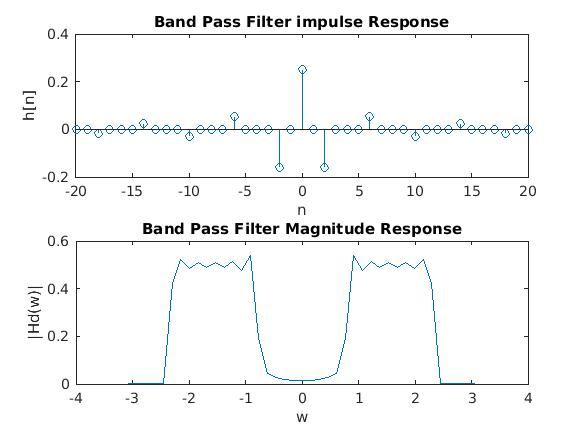
\includegraphics[scale = .5]{1_bpf_20}
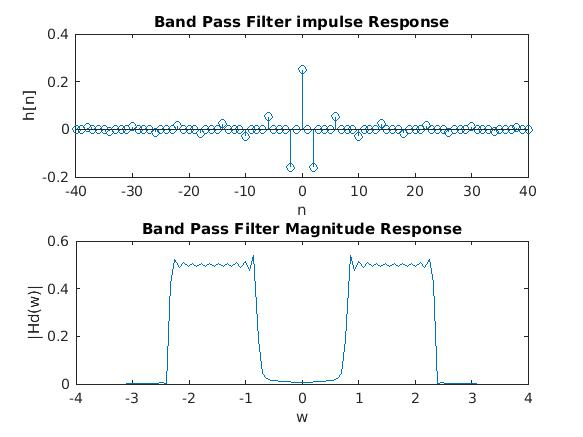
\includegraphics[scale = .5]{1_bpf_40}
\end{figure}


\begin{figure}[H]
\color{red}
\underline{\textbf{Report Item 2}}
\color{black}
\lstinputlisting[language=Matlab]{impresp.m}
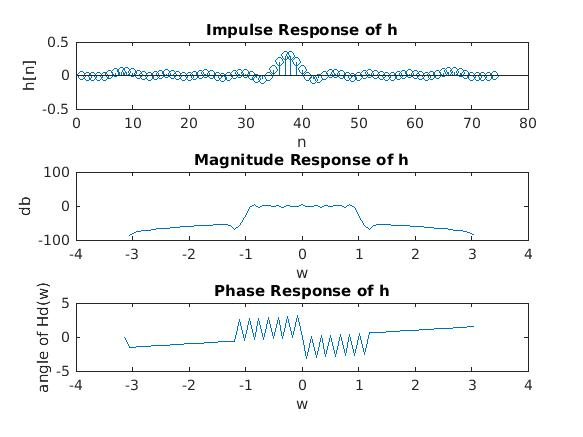
\includegraphics[scale = .5]{report2}
\\The transition bandwidth is around .5 radians wide. I calculated the maximum passband ripple(max - min) to be around 8db. The stopband ripple(max - min) seems to be around 20db.
\end{figure}

\begin{figure}[H]
\color{red}
\underline{\textbf{Report Item 3}}
\color{black}
\lstinputlisting[language=Matlab]{FIR_FILTER.m}
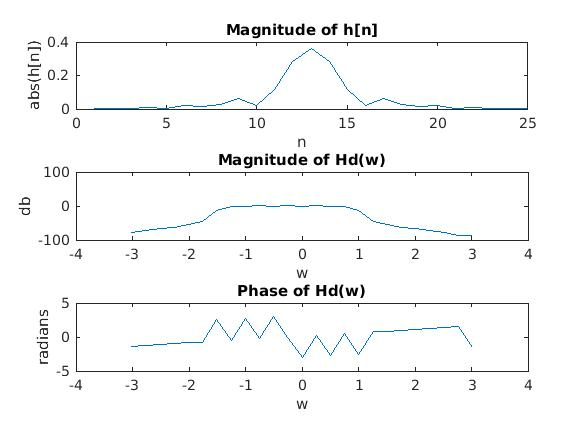
\includegraphics[scale = .5]{report3}
\\The passband ripple apears to be about 5db, stopband, about 25db. The passband edge frequency is 0.9 radians and the stopband edge frequency is about 1.2 radians.
\end{figure}

\begin{figure}[H]
\color{red}
\underline{\textbf{Report Item 4}}
\color{black}
\lstinputlisting[language=Matlab]{report4.m}
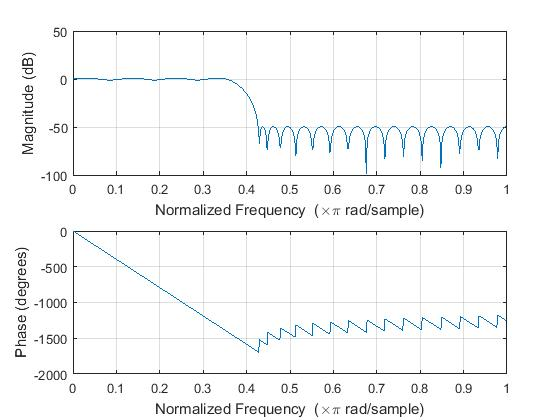
\includegraphics[scale = .5]{report4}
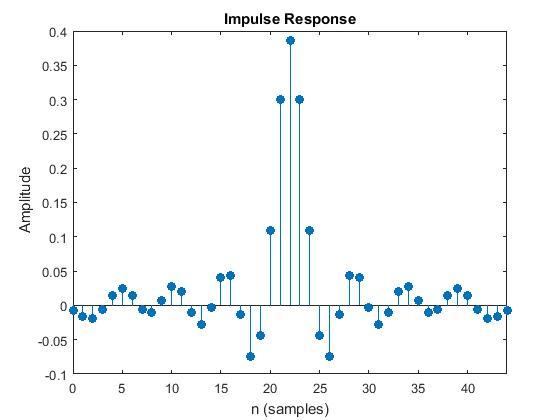
\includegraphics[scale = .5]{report4i}
\end{figure}

\begin{figure}[H]
\color{red}
\underline{\textbf{Report Item 5}}
\color{black}
\lstinputlisting[language=Matlab]{mySTDFT.m}
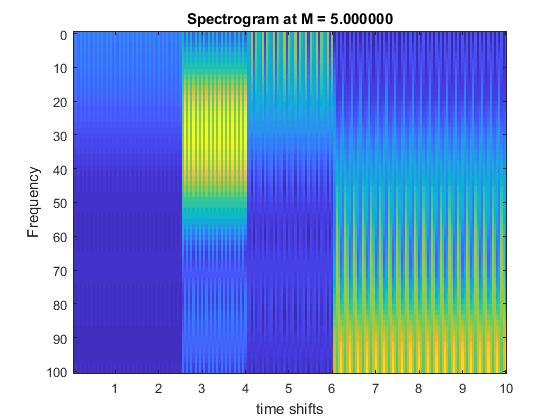
\includegraphics[scale = .5]{report5}
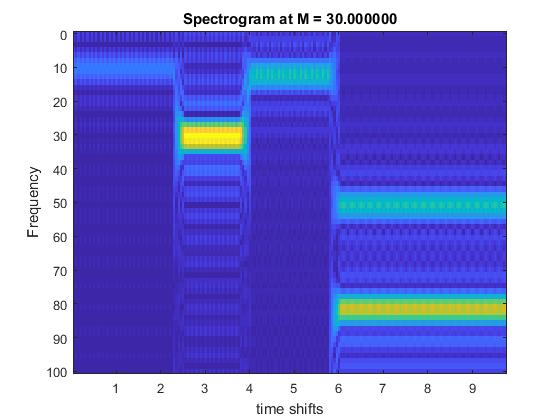
\includegraphics[scale = .5]{report5_2}
\end{figure}
\begin{figure}[H]
\\By the spectrogram we can see that(M = 5) there are frequencies ranging from 10 to 50 hz at 2.5 to 4 seconds. Then there are also 80 to 100 hz at 6 to 10 seconds. With M =30, We see frequencies 10hz at 1:2 seconds, 20hz at 2.5:4 seconds, 10hz at 4:6 seconds, and 50 and 85 hz at 6:10 seconds. When we increase M to 30 our minimum frequency to be distinguished goes down and therefore the frequency bands are more distinguishable. Note that $N\Delta t = \frac{1/fmin}$, increasing N will decrease fmin.
\end{figure}

\begin{figure}[H]
  \color{red}
  \underline{\textbf{Report Item 6}}
  \color{black}
\lstinputlisting[language=Matlab]{report6.m}
\\ The audio file when played at real time is 15 seconds.
\end{figure}

\begin{figure}[H]
Before filter, I used paramaters $M = 5000$, $P = 1024$, $D = 5$. The signal and sampling frequency are given to us.
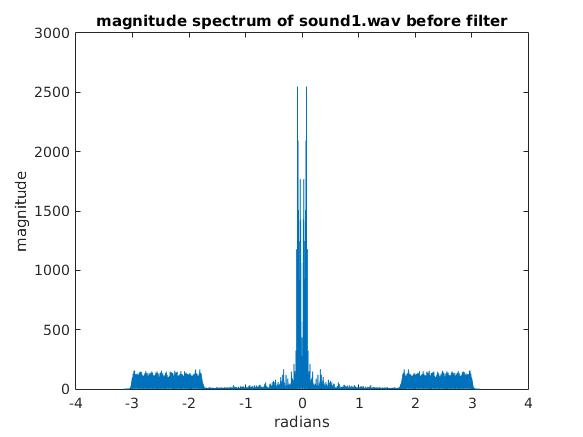
\includegraphics[scale = .5]{report6_1}
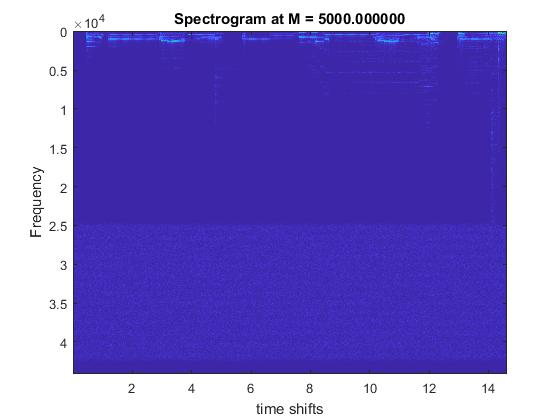
\includegraphics[scale = .5]{report6_2}
\end{figure}

\begin{figure}[H]
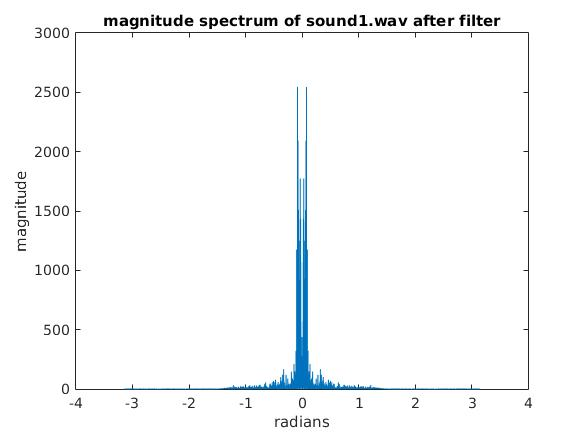
\includegraphics[scale = .5]{report6_3}
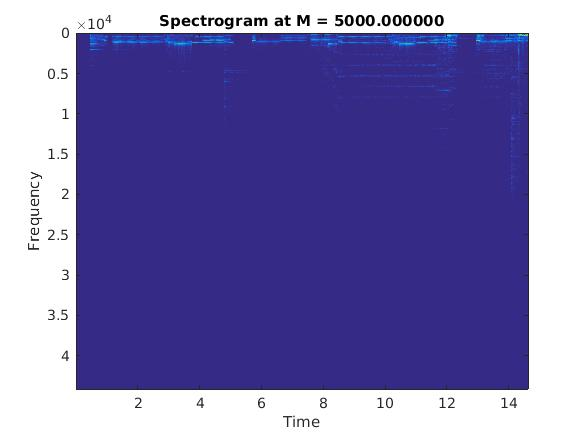
\includegraphics[scale = .5]{report6_4}
\\ Notice that noise in the higher frequencies of the spectrogram are cleaned. Because the frequencies are mutally exclusive, the filter works well.
\end{figure}

\begin{figure}[H]
\color{red}
\underline{\textbf{Report Item 7}}
\color{black}
\lstinputlisting[language=Matlab]{report7.m}
\end{figure}

\begin{figure}[H]
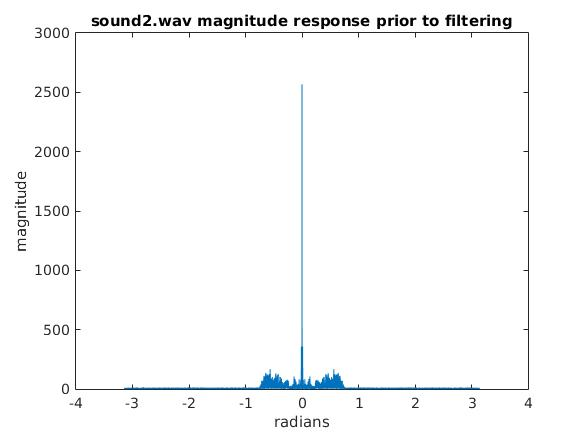
\includegraphics[scale = .5]{report7_1}
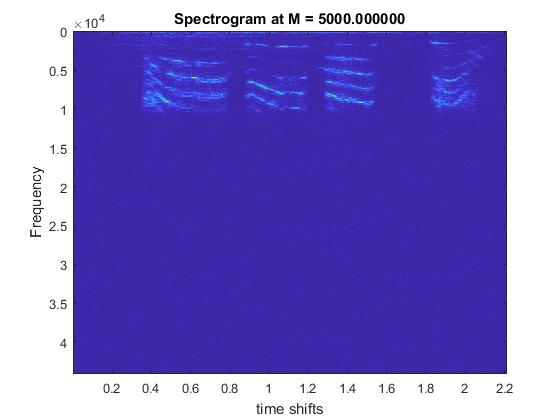
\includegraphics[scale = .5]{report7_2}
\\Before filter, I used paramaters $M = 5000$, $P = 1024$, $D = 5$. The signal and sampling frequency are given to us.
In the spectrogram we can see noise distributed among the low frequency bands.
\end{figure}

\begin{figure}[H]
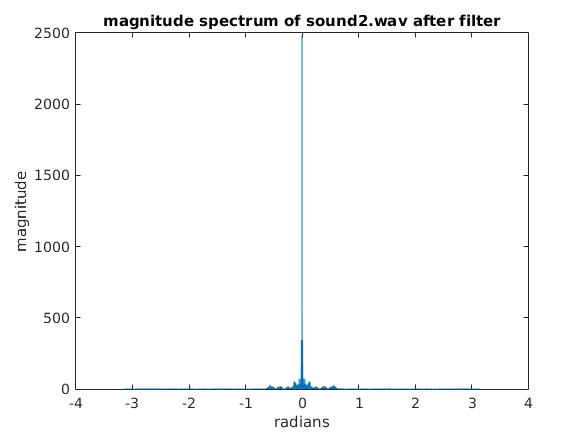
\includegraphics[scale = .5]{report7_3}
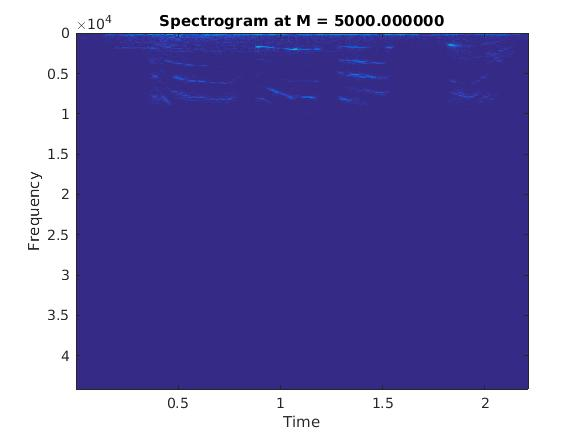
\includegraphics[scale = .5]{report7_4}
\\ I tried to filter out all of the noise outside of the lowest frequency but with such a small band of desired frequency, creating a sinc of that small width is hard. Therefore some noise still remains.
Also, the desired sound is quieter after filtering. Overall, the filter helped, but could be better.
\end{figure}

\begin{figure}[H]
\lstinputlisting[language=Matlab]{report8.m}
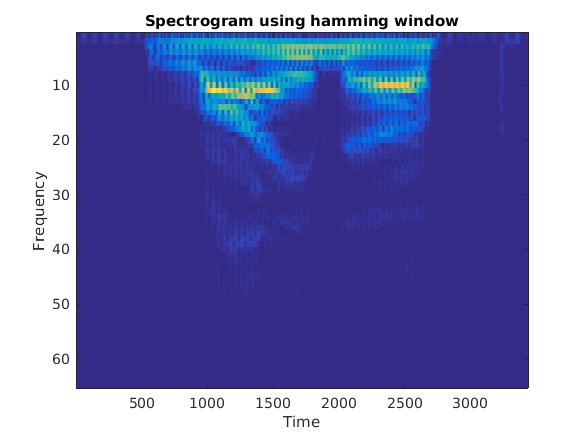
\includegraphics[scale = .5]{report8_1}
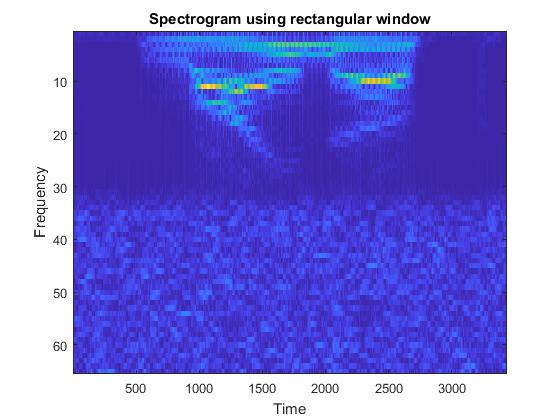
\includegraphics[scale = .5]{report8_2}
\\
\end{figure}

\end{document}
